\subsection{Mixed Gain-Phase Stability Criterion}
\begin{figure}[t]
    \centering
    \begin{subfigure}{0.45\columnwidth}
        \centering
        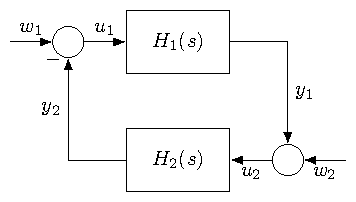
\includegraphics[width=\linewidth]{feedback_diagram.pdf}
        \caption{Generic Feedback System}
        \label{fig:fd_diagram}
    \end{subfigure}
    \begin{subfigure}{0.45\columnwidth}
        \centering
        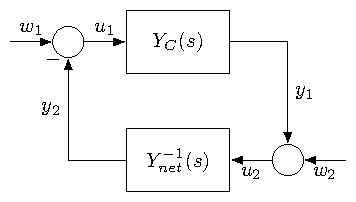
\includegraphics[width=\linewidth]{feedback_diagram_converters.pdf}
        \caption{Admittance Feedback}
        \label{fig:fd_diagram_conv_net}
    \end{subfigure}
    \caption{Diagram of the feedback connection.}
    \label{fig:twoside}
    \vspace{-1em}
\end{figure}
The concepts introduced above provide a framework for assessing the stability of linear time-invariant systems. Consider the feedback interconnection of $H_1(s)$ and $H_2(s)$ shown in Figure \ref{fig:fd_diagram}. 
The following theorem gives a sufficient condition for the stability of the resulting closed-loop system \cite{zhao2022smallgainmeetssmall}.
\begin{thm}[Mixed Small Gain-Phase Theorem]
    Let the open-loop systems $H_1, H_2$ be real, rational, stable, and proper transfer function matrices. Then, the closed loop system is stable if for each $\omega \in [0, \infty]$, either
    \begin{enumerate}
        \item The product of the maximum singular values satisfies:
        \begin{equation*}
            \overline{\sigma}(H_1(j\omega))\overline{\sigma}(H_2(j\omega))<1
        \end{equation*}
        \item 
        or $H_1(j\omega)$ is semi-sectorial and $H_2(j\omega)$ is sectorial, and
        \begin{equation*}
            \overline{\phi}(H_1(j\omega))+\overline{\phi}(H_2(j\omega))<\pi
        \end{equation*}
        \begin{equation*}
            \underline{\phi}(H_1(j\omega))+\underline{\phi}(H_2(j\omega))>-\pi
        \end{equation*}
    \end{enumerate}
    \label{thm:mixed_small_gain_phase}
\end{thm}
This theorem unifies the traditional small-gain condition and its phase counterpart into a single stability framework, enabling the use of either gain-based or phase-based bounds at each frequency, depending on which provides a less conservative estimate.

\subsection{Decentralized condition for power system stability}
In the context of power systems, we are interested in assessing the stability of the interconnection of $n$ power electronic converters to a given network. 
Let 
\begin{equation}
    \mathbf{Y}_C(s)=\text{diag}(Y_{C_1}(s),Y_{C_2}(s),\cdots,Y_{C_n}(s))
    \label{eq:block_diagonal}
\end{equation}
denote the overall converter admittance matrix, where $Y_{C_i}(s)$ represents the admittance of the $i$-th converter. Let $\mathbf{Y}_{net}(s)$ denote the network admittance. In this work, $\mathbf{Y}_{net}(s)$ is assumed to be the Kron-reduced network, where all internal nodes that are not connected to any converter are eliminated. All admittances are expressed in a common global $dq$ reference frame. Analogous to Figure \ref{fig:fd_diagram},  the interconnection between the converters and the network can be represented as the feedback loop shown in Figure \ref{fig:fd_diagram_conv_net}.

Theorem \ref{thm:mixed_small_gain_phase} can be applied directly to this system to provide a stability condition. However, the block-diagonal structure of $\mathbf{Y}_C(s)$ allows a decentralized stability analysis, leading to the following result \cite{huangGainPhaseDecentralized2024}.

\begin{thm}[Decentralized Mixed Small Gain-Phase Theorem]
    The multi-converter system in Figure \ref{fig:fd_diagram_conv_net} is stable if the open-loop systems are stable, and for each $\omega \in [0,\infty]$, either
    \begin{enumerate}
        \item 
        the decentralized gain condition, i.e.,
        \begin{equation*}
            \max_i \overline{\sigma}(Y_{C_i}(j\omega))<\underline{\sigma}(\mathbf{Y}_{net}(j\omega))
        \end{equation*}
        %\vspace{-1em}
        holds, or
        \item 
        the decentralized phase condition, i.e
        every $Y_{C_i}(j\omega)$ is quasi-sectorial, and $\mathbf{Y}_{net}(j\omega)$ is sectorial, and
        \begin{equation*}
            \max_i\overline{\phi}(Y_{C_i}(j\omega))<\pi-\overline{\phi}(\mathbf{Y}_{net}^{-1}(j\omega)),
        \end{equation*}
        \vspace{-1.85em}
        \begin{equation*}
            \min_i\underline{\phi}(Y_{C_i}(j\omega))>-\pi-\underline{\phi}(\mathbf{Y}_{net}^{-1}(j\omega))
        \end{equation*}
        \vspace{-2em}
    \end{enumerate}
    \label{thm:dec_mixed_small_gain_phase}
\end{thm}
This decentralized formulation allows the stability of a large-scale multi-converter system to be certified by verifying local conditions on each converter model together with the network model, without requiring the explicit computation of the full interconnected system’s dynamics.